\documentclass[12pt]{article}
\usepackage{preamble}

\pagestyle{fancy}
\fancyhead[LO,LE]{Теория вероятности}
\fancyhead[CO,CE]{05.11.2024}
\fancyhead[RO,RE]{Лекции Блаженова А. В.}

\fancyfoot[L]{\scriptsize исходники найдутся тут: \\ \url{https://github.com/pelmesh619/itmo_conspects} \Cat}

\begin{document}
    \subsection{Преобразование случайных величин}

    \subsubsection{Стандартизация случайной величины}

    \Def Пусть имеется случайная величина $\xi$. Соответствующей ей стандартной величиной называется
    случайная величина $\eta = \frac{\xi - E\xi}{\sigma}$

    \textbf{Свойства}:

    $E\eta = 0; D\eta = 1$

    \begin{MyProof}
        $E\eta = E \frac{\xi - E\xi}{\sigma} = \frac{1}{\sigma} (E\xi - E\xi) = 0$

        $D\eta = D \frac{\xi - E\xi}{\sigma} = \frac{1}{\sigma^2} D\xi = 1$
    \end{MyProof}

    Стандартизованная случайная величина не имеет единиц измерения, таким образом, ее свойства от них не зависят

    \mediumvspace

    \underline{Задача}: пусть имеется функция $g(x)$ и случайная величина $\xi$, $\eta = g(\xi)$. Определить ее характеристики

    \Nota Если $\xi$ - дискретная случайная величина, то ее законы распределения находятся просто: значения $x_i$ в верхней строке заменяем $g(x_i)$, вероятности остаются прежние.
    Поэтому будем рассматривать непрерывной случайной величины $\xi$

    \Notas Возможна ситуация, когда $\xi$ - абсолютно непрерывная случайная величина, $g(x)$ - непрерывна, но $g(\xi)$ имеет дискретное распределение

    \subsubsection{Линейное преобразование}

    \begin{MyTheorem}
        \Ths Пусть $\xi$ имеет плотность $f_\xi(x)$, тогда $\eta = a\xi + b$, где $a \neq 0$, имеет плотность $f_\eta(x) = \frac{1}{|a|}f_\xi(\frac{f - b}{a})$
    \end{MyTheorem}

    \begin{MyProof}
        Пусть $a > 0$, тогда $F_\eta(x) = p(\eta < x) = p(a\xi + b < x) = p(\xi < \frac{x - b}{a}) = \int_{-\infty}^{\frac{x - b}{a}} f_\xi(t) dt = 
        \left[\begin{matrix}t = \frac{y - b}{a} & dt = \frac{1}{a} dy & y = at + b \\ y(-\infty) = -\infty & y(\frac{x - b}{a}) = x\end{matrix}\right] = 
        \int_{-\infty}^x \frac{1}{a} f_\xi(\frac{y - b}{a}) dy \Longrightarrow \eta = \frac{1}{|a|} f_\xi (\frac{x - b}{a})$

        Пусть $a < 0$, тогда $F_\eta(x) = p(\eta < x) = p(a\xi + b < x) = p(\xi > \frac{x - b}{a}) = \int_{\frac{x - b}{a}}^{\infty} f_\xi(t) dt = 
        \left[\begin{matrix}t = \frac{y - b}{a} & dt = \frac{1}{a} dy & y = at + b \\ y(\infty) = -\infty & y(\frac{x - b}{a}) = x\end{matrix}\right] = 
        -\int_{-\infty}^x \frac{1}{a} f_\xi(\frac{y - b}{a}) dy \Longrightarrow \eta = \frac{1}{|a|} f_\xi (\frac{x - b}{a})$
    \end{MyProof}

    \underline{Следствие}

    1) Если $\xi \in N(a, \sigma^2)$, то $\eta = \gamma \xi + b \in N(a\gamma + b; \gamma^2 \sigma^2)$

    \begin{MyProof}
        Так как $\xi \in N(a, \sigma^2)$, то $f_\xi(x) = \frac{1}{\sigma\sqrt{2\pi}} e^{-\frac{(x - a)}{2\sigma^2}}, x \in \Real$

        Тогда $f_\eta(x) = \frac{1}{|\gamma|} \cdot \frac{1}{\sigma\sqrt{2\pi}} e^{-\frac{(\frac{x - b}{\gamma} - a)^2}{2\sigma^2}} = \frac{1}{|\gamma|\sigma\sqrt{2\pi}} e^{-\frac{(x - b - a\gamma)^2}{2\sigma^2\gamma^2}} \Longrightarrow \eta \in N(b + a\gamma; \sigma^2\gamma^2)$
    \end{MyProof}

    2) Если $\eta \in N(0, 1)$ - стандартное нормальное распределение, то $\xi = \sigma \eta + a \in N(a, \sigma^2)$

    3) Если $\eta \in U(0, 1)$ - стандартное равномерное распределение и $a > 0$, то $\xi = a\eta + b \in U(b, a + b)$

    4) Если $\xi \in E_\alpha$, то $\alpha \xi \in E_1$

    \subsubsection{Монотонное преобразование}

    \begin{MyTheorem}
        \Ths Пусть $f_\xi(x)$ - плотность случайной величины $\xi$, $g(x)$ - строго монотонная функция. Тогда 
        случайная величина $\eta = g(\xi)$ имеет плотность

        \[f_\eta(x) = |h^\prime(x)| f_\xi(h(x)), \qquad\qquad \text{где } h(g(x)) = x\]
    \end{MyTheorem}

    Если $g(x)$ не является монотонное функцией, то поступаем следующим образом: разбиваем $g(x)$ на интервалы монотонности, 
    для каждого $i$-ого интервала находимся $h_i(x)$ и плотность случайной величины ищем по \textit{формуле Смирнова}: 
    $f_\eta(x) = \sum_{i = 0}^n |h_i^\prime(x)| f_\xi(h_i(x))$
    
    \subsubsection{Квантильное преобразование}

    \begin{MyTheorem}
        \ThNs{1} Пусть функция распределения случайной величины $\xi$ $F_\xi(x)$ - непрерывная функция. 
        Тогда $\eta = F(\xi) \in U(0, 1)$ - стандартное равномерное распределение
    \end{MyTheorem}

    \begin{MyProof}
        Ясно, что $0 \leq \eta \leq 1$

        a) $F(x)$ - строго возрастающая функция. Тогда $\exists F^{-1}(x)$ - обратная, $F_\eta(x) = p(\eta < x) = p(F(\xi) < x) = 
        \begin{cases}0, & x < 0 \\ p(\xi < F^{-1}(x)) = F(F^{-1}(x)) = x, & 0 \leq x \leq 1 \text{ - функция распределения } U(0, 1) \\ 1, & x > 1 \end{cases}$

        б) $F(x)$ - не является строго возрастающей функцией - то есть существуют участки постоянства, в этом случае
        определим $F^{-1}$ как $F^{-1}(x) = \min_{t} (t \ | \ F(t) = x)$ - то есть берем самую левую точку такого интервала

        Тогда снова будет при $0 \leq x \leq 1 \ F_\eta(x) = p(\eta < x) = p(F(\xi) < x) = F(F^{-1}(x)) = x$

    \end{MyProof}

    Сформулируем обратную теорему: пусть $F(x)$ - функция распределения (необязательно непрерывная) случайной величины $\xi$,
    обозначим $F^{-1}(x) = \inf_t (t \ | F(t) \geq x)$.

    В случае непрерывной $F(x)$ это определение совпадет с предыдущем

    \begin{MyTheorem}
        \ThNs{2} Пусть $\eta \in U(0, 1)$ - стандартное равномерное распределение, $F(x)$ - произвольная функция распределения. 
        Тогда $\xi = F^{-1}(\eta)$ имеет функцию распределения $F(x)$
    \end{MyTheorem}

    Данное преобразование $\xi = F^{-1}(\eta)$ называют квантильным

    Доказательство аналогично предыдущей теореме
    
    Смысл: датчики случайных чисел имеют стандартное равномерное распределение, из теоремы следует, что при помощи
    датчика случайных чисел и квантильного преобразования мы сможем смоделировать любое нужно распределение

    \ExN{1} Смоделируем показательное распределение $E_\alpha: \ F_\alpha(x) = \begin{cases}0, & x < 0 \\ 1 - e^{-\alpha x}, & x \geq 0\end{cases}$

    $\eta = 1 - e^{-\alpha x}, \ e^{-\alpha x} = 1 - \eta, \ x = -\frac{1}{\alpha} \ln(1 - \eta)$ - функция, обратная к $F_\alpha(x)$

    Если $\eta \in U(0, 1)$, то $\xi = -\frac{1}{\alpha} \ln(1 - \eta) \in E_\alpha$

    \ExN{2} $\xi \in N(0, 1), \ F_0(x) = \frac{1}{\sqrt{2\pi}} \int_{-\infty}^x e^{-z^2}{2} dz$

    Пусть $F_0^{-1}(x)$ - функция обратная к $F_0(x)$

    Если $\eta \in U(0, 1)$, то $F_0^{-1}(\eta) \in N(0, 1)$

    \subsection{Характеристики преобразованной случайной величины}

    \begin{MyTheorem}
        \Ths Если $\xi$ - дискретная случайная величина, то $Eg(\xi) = \sum_{i = 1}^\infty g(x_i) \cdot p_i = \sum_{i = 1}^\infty g(x_i) \cdot p(\xi = x_i)$

        Для непрерывной случайной величины $Eg(\xi) = \int_{-\infty}^{\infty} g(x) f_\xi(x) dx$
    \end{MyTheorem}

    \subsubsection{Свойства моментов}

    1) Если $\xi \geq 0$, то $E\xi \geq 0$

    2) Если $\xi \leq \eta$, то $E\xi \leq E\eta$

    \begin{MyProof}
        $\xi \leq \eta \Longrightarrow \eta - \xi \geq 0 \Longrightarrow E(\eta - \xi) \geq 0 \Longrightarrow E\eta - E\xi \geq 0 \Longrightarrow E\eta \geq E\xi$
    \end{MyProof}

    3) Если $|\xi| \leq |\eta|$, то $E|\xi|^k \leq E|\eta|^k$

    4) Если существует момент $m_t$ случайной величины $\xi$, то существует $m_s$ при $s < t$ (при условии, что интеграл/сумма сходятся)

    \begin{MyProof}
        Пусть $s < t$. Тогда $|x|^s \leq \min(1, |x|^t) \leq 1 + |x|^t$, так как при $|x| < 1, \ |x|^s \leq 1$ и при $|x| \geq 1, \ |x|^s \leq |x|^t$
    
        $E|\xi|^s \leq E|\xi|^t + 1$ и если $E|\xi|^t$ существует (конечно), то $\exists E|\xi|^s$
    
    \end{MyProof}

    \begin{MyTheorem}
        \ThNs{Неравенство Йенсена} Пусть функция $g(x)$ выпукла вниз, тогда для любой случайной величины $\xi$

        \[Eg(\xi) \geq g(E\xi)\]
    \end{MyTheorem}

    \Nota Если $g(x)$ выпукла вверх, знак неравенства меняется
    
    \begin{MyProof}
        Если $g(x)$ выпукла вниз, то в любой ее точке, можно провести прямую, лежащую не выше графика функции. То есть для 
        любой $x_0$ существует $k(x_0)$ такой, что $g(x) \geq g(x_0) + k(x_0) (x - x_0)$

        Пусть $x_0 = E\xi$, $g(E\xi) \geq g(E\xi) + k(E\xi) (x - E\xi)$

        $Eg(\xi) \geq Eg(E\xi) + k(E\xi) \underset{= 0}{(E\xi - E\xi)}$

        $Eg(\xi) \geq g(E\xi)$
    \end{MyProof}

    % ниче не понял, maybe wrong

    Следствие:

    $Ee^\xi \geq e^{E\xi}, \quad E\xi^2 \geq (E\xi)^2, \quad E|q| \geq |Eq|, \quad E\ln(\xi) \leq \ln(E\xi), \quad E\frac{1}{\xi} \geq \frac{1}{E\xi}$ при $\xi > 0$


    \begin{minipage}{\textwidth}
        \begin{wrapfigure}{r}{0pt}
            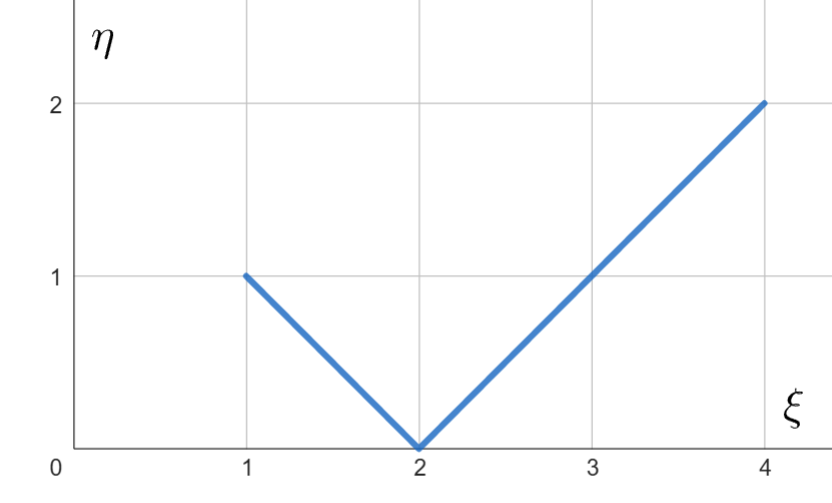
\includegraphics[width=7cm]{probtheory/images/probtheory_2024_11_05_1}
        \end{wrapfigure}

        \Ex на формулу Смирнова: дана плотность распределения
    
        $f_\xi(x) = \begin{cases}0, & x < 1 \\ \frac{4}{3x^2}, & 1 \leq x \leq 4, 0 & x > 4\end{cases}$
    
        Найти $f_\eta$ для $\eta = |\xi - 2|$

        \underline{Решение}

        $\xi \in [1, 4], \quad \eta \in [0, 2]$
    \end{minipage}

    \begin{cases}
        0 \leq \eta \leq 1 \Longrightarrow h_1(\eta) = \eta + 2 \text{ и } h_2(\eta) = 2 - \eta & \text{\qquad - 2 ветви} \\ 
        1 < \eta \leq 2 \Longrightarrow h_1(\eta) = \eta + 2 & \text{\qquad - 1 ветвь}
    \end{cases}

    $h_1^\prime(\eta) = 1, h_2^\prime(\eta) = -1 \qquad |h_1^\prime(\eta)| = |h_2^\prime(\eta)| = 1$

    $f_\eta(x) = \sum_i |h_i^\prime(x)| f_\xi(h_i(x))$

    $f_\eta(x) = \begin{cases}0, & x < 0 \\ \frac{4}{3}\left(\frac{1}{(x + 2)^2} + \frac{1}{(2 - x)^2}\right), & 0 \leq x \leq 1 \\ \frac{4}{3}\frac{1}{(x + 2)^2}, & 1 < x \leq 2 \\ 0 & x > 2\end{cases}$

\end{document}
